\section{Принцип индукции}

Пусть $P(n)$~--- некоторое утвержение, в котором как-то фигурирует натуральное число $n$. Пусть нам удалось доказать истинность $P(0)$, а так же следствие $P(n)\to P(n+1)$ для любого $n$. Используя это следствие, мы можем получить $P(0)\to P(1)$. Отсюда, опять же по тому же следствию $P(1)\to P(2)$. Затем $P(2)\to P(3)$. Продолжая так бесконечно долго, мы получаем, что утверждение истинно вообще для любого натурального $n$.

Приведенное рассуждение довольно неформально, фраза <<продолжая так бесконечно долго>> явно требует уточнения. Буквально через несколько абзацев мы передокажем этот принцып строго, а пока рассмотрим пример, который должен дать нам интуицию о том, как этот принцип вообще предполагается использовать. Обозначим
$$S(n) = 1 + 2 +3 \ldots + n$$
и
$$S'(n) = {n(n+1)\over 2}$$
Доказываемое утверждение $P$ будет состоять в том, что
$$S(n) = S'(n)$$
то есть что две приведенные две формулы эквивалентны.

Равенство $S(0) = S'(0)$ довольно очевидно, нам теперь надо доказать импликацию $P(n)\to P(n + 1)$, то есть доказать, что если эти формулы совпадают для произвольного $n$, то они будут совпадать и для $n + 1$. В соответствии с определением для любого $n$
$$S(n + 1) = 1 + 2 + \ldots + n + (n + 1)$$
Из предположения о том, что утверждение верно для $n$, мы первые $n$ слагаемых можем переписать, используя формулу для $S'$:
\begin{align*}
S(n + 1) &= {n(n + 1)\over 2} + (n + 1)\\
	&= {n^2 + n\over 2} + {2n + 2\over 2} \\
	&= {n^ 2 + 3n + 2 \over 2} \\
	&= {(n + 1)(n + 2)\over 2} \\
	&= {S'(n + 1)}
\end{align*}

Всё! Мы доказали, что из равенства $S(n)=S'(n)$ следует так же равенство $S(n+1)=S'(n+1)$, а это всё что требуется: теперь принцип индукции гарантирует нам, что действительно для любого $n$ эти формулы совпадают.

Принцип индукции чрезвычайно силён: подаляющее большинство теорем, в которых как-то фигурируют произвольные натуральные числа, могут быть доказаны таким образом, причем во многих случаях доказательство оказывается не сложным. С другой стороны этот метод обладает и явным недостатком: он позволяет нам доказать утверждение, которое нам уже известно, но не даёт никакого способа это утверждение вывести, не зная ответа. Например, если бы задача изначально стояла не в том, чтобы доказать равенство двух формул, а в том, чтобы получить краткое выражение для $S(n)$, метод индукции нам уже почти никак не помог бы.

Часто о решении можно догадаться. Например, если записать первые значения $S(n)$
$$0, 1, 3, 6, 10, 15, 21, 28, 36, \ldots$$
то о формуле для $S(n)$ можно догадаться. По крайней мере так пишут в учебниках, что догадаться можно, а в жизни я людей, которые легко улавливают такие закономерности, видел очень мало. Но предположим, что догадаться можно.

Часто формулу можно подобрать. Для $S(n)$ мы могли бы предположить, что формула имеет вид
$S(n) = {an^2 + bn + c\over d}$
где $a, b, c, d$~--- некоторые неизвестные нам числа. Затем, вычислив явно значения $S(0), S(1), S(2), S(3)$ можно убедиться в том, что единственными вариантом, который работает, является набор значений
$$a=1, b=3, c=2, d=2$$
Эти значения приводят к формуле $S'(n)$, но это пока не является доказательством, поскольку мы проверили эту формулу лишь на четырёх значениях $n$, но по крайней мере нам уже есть к чему приложить принцип индукции.

Этот подход может показаться так же сложным и надуманным, но на самом деле он довольно прост. Если нарисовать значения $S(n)$ на графике, то их расположение будет очень сильно похоже на параболу, которую тут же распознает любой смышленный школьник, а формула с неизвестными, которую я привёл выше~--- это как раз формула параболы в общем виде. Мы пока не рассматривали графики функций, поэтому такое рассуждение может показаться сложным или необычным, но через какое-то время вы научитесь довольно быстро искать такие решения самостоятельно.

Тем не менее даже если мы формулу каким-то образом подобрали, а потом доказали её, нам хочется её еще и понять. Да, мы знаем, что $S(n)=S'(n)$, но с какой стати? Эти две формулы совершенно не похожи друг на друга и их взаимосвязь совершенно не ясна. Это главная проблема принципа индукции: он позволяет доказать очень многое, но он совершенно не проясняет ситуацию.

Попробуем вывести краткую формулу для $S(n)$ совершенно другим способом. Для этого вначале расположим красные квадраты в ряды один под другим (рис.3.8). В первом ряду у нас будет один квадрат, во втором два, в третьем три и так далее. Наша задача~--- подсчитать сколько всего получается квадратов, если мы располагаем таким образом квадраты в $n$ строчках. Как видно из картинки, эти квадраты образуют некое подобие треугольника, поэтому такие числа называются \term{треугольными}.

\begin{figure}[h]
\centering
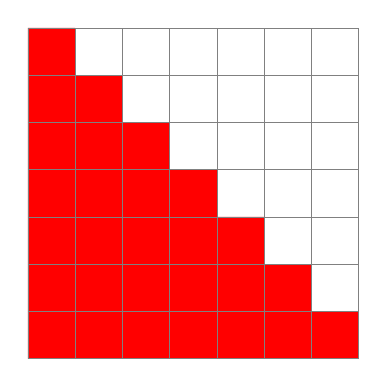
\begin{tikzpicture}
  \fill[red] (0, 0) -- (4.2cm, 0) -- (4.2cm, .6cm) -- (3.6cm, .6cm) -- (3.6cm, 1.2cm) -- (3cm, 1.2cm) -- (3cm, 1.8cm) -- (2.4cm, 1.8cm) -- (2.4cm, 2.4cm) -- (1.8cm, 2.4cm) -- (1.8cm, 3cm) -- (1.2cm, 3cm) -- (1.2cm, 3.6cm) -- (.6cm, 3.6cm) -- (.6cm, 4.2cm) -- (0, 4.2cm) -- cycle;
  \draw[step=.6cm,gray,very thin] (0, 0) grid (4.2cm,4.2cm);
\end{tikzpicture}
\caption{Треугольные числа}
\end{figure}

Помимо квадратов я изобразил сетку, одна ячейка которой по размеру равняется величине квадрата, а строк и колонок в ней равно $n$. Всего клеток, таким образом, имеется $n^2$. Из всех этих клеток красные клетки~--- это те, что лежат на диагонале (их $n$ штук), а так же половина от оставшихся клеток. Итого, мы получаем
$$S(n) = {n^2 - n\over 2} + n = {n^2 - n + 2n \over 2} = {n(n+1)\over 2}$$
Без каких-либо хитрых умоизысканий мы получили ту же самую формулу, причем теперь нам вполне понятно откуда она взялась и что означает.

В этом примере метод индукции оказался одновременно и сложнее и менее информативным~--- последний метод показал нам общую идею откуда такая идея берется, а не просто дал доказательство. Часто именно так и происходит, поэтому мы чаще всего будем избегать и приводить по возможности методы, которые как-то раскрывают суть теоремы, а не просто формально её доказывать лишь бы доказать.

Тем не менее, последнее доказательство с клетками в строгом смысле доказательством не является. Как мы уже говорили в первой главе, строгое доказательство~--- это последовательность предложений, выводимых из аксиом с использованием четко определенного набора правил. Доказательство с клетками далеко от такого принципа: мы не определили никаких геометрических понятий, мы никак не определили по какому вообще критерию мы отождествляем клетки с числами, мы никак даже не определяем понятие положения клеток в пространстве. Безусловно, доказательство выглядит убедительным (и, пролив много пота и крови, его можно сделать абсолютно строгим) и у большинства людей оно справедливо не будет вызывать сомнений. Однако формально этого не достаточно: многие учителя (не самые умные представители) в университетах такие доказательства не примут, так же подобное доказательство не признают многие авторы учебников, и всюду доказывают любую мелочь по индукции. Я считаю это неправильным (правда, я и образования не получил), поэтому мы будем по возможности избирать не всегда самый формально корректный, но по возможности самый содержательный метод доказательства.

Но это мы уже отвлеклись на лирику. Метод индукции требует строгого обоснования, так давайте это обоснование предъявим.

Предположим, что мы доказали истинность $P(0)$ и импликацию $P(n)\to P(n+1)$. Предположим, что всё таки метод индукции врёт, и есть такие числа, для которых утверждение $P$ ложно. Множество таких чисел обозначим за $X\subset \mathbb{N}$. Как мы уже говорили в первом параграфе, это множество имеет наименьший элемент, который мы обозначим за $m$. Однако в этом случае $P(m-1)$ должно быть истинно, и из ипликации $P(m-1)\to P(m)$ мы приходим к противоречию. Значит, $X=\emptyset$, что и требовалось доказать.

Метод индукции можно обобщить двумя способами. Во-первых, мы могли бы начинать наш отсчет не с P(0), а с произвольного элемента $P(k)$. На доказательство и общий принцип применения индукции это никак не повлияло бы, поэтому мы не будем рассматривать этот случай.

Второе обобщение индукции заключается в том, что вместо импликаии $P(n)\to P(n+1)$ мы могли бы рассматривать импликацию $(\forall m<n, P(m))\to P(n)$. Здесь мы в доказательстве опираемся не только на одно значение $n$, но на все значения, меньшие заданного, для которых уже доказана истинность $P(m)$. Справедливость такого принципа индукции доказывается аналогично: если бы было множество чисел $X$, для которых утверждение неверно, мы могли бы взять минимальный элемент этого множества $m$, а отсюда мы сразу же приходим к противоречию как и в первом случае.

Первоначальный подход называется \term{слабой индукцией}, последний подход называется \term{сильной индукцией}. Если рассматривать только натуральные числа, то разница между ними не велика. Слабая индукция следует из сильной при замене $\forall m<n P(m)$ на $P(n-1)$, сильная индукция может получиться из слабой, если ввести множества
$$A_i = \{0, 1, 2, \ldots, i\}$$
и доказывать используя слабую индукцию утверждение
$$P'(n) = \forall x \in A_n, P(x)$$
вместо первоначального $P(n)$.

Если однако выйти за рамки натуральных чисел, то окажется, что сильная индукция всё же действительно сильнее слабой. Подробно мы такие конструкции будем рассматривать в шестой главе, но сейчас мы уже можем показать пример, который даст нам представление о том, что же было не правильно в первоначальном рассуждении в начале параграфа.

Рассмотрим множество $\mathbb{N}^2$, упорядоченное лексикографически. Напомню, что это значит, что мы рассматриваем пары натуральных чисел $(a, b)$, а для сравнения на больше и меньше используем тот же принцип, по которому упорядочены слова в алфавите: вначале мы сравниваем первые числа, и только если они равны, то сравниваем пторые числа. Так
$$(1, 2) < (10, 1)$$
$$(4, 4) > (4, 1)$$

Как и натуральные числа, это множество является вполне упорядоченным и мы легко можем выбрать из любого подмножества минимальный элемент (проверьте!). Пусть теперь для некоторого утверждения $P(n)$ найдётся непустое множество элементов $X$, для которых $P(n)$ не выполняется, и $m=\min X$.

Предположим сначала, что мы доказали предположение сильной индукции. Тогда $(\forall n < m, P(n))\to P(m)$, и это приводит к противоречию. Значит, $P(n)$ всё же справедливо в этом случае для всех $n$.

Теперь предположим, что мы доказали только предположение слабой индукции $P(n)\to P(n+1)$. Поскольку $m$ теоретически может быть произвольным, выберем в качетсве его значения элемент $(1, 0) \in \mathbb{N}^2$. Любой элемент, меньший такого $m$ имеет вид $(0, k)$, причем таких элементов бесконечно много. Это значит, что мы никаким образом не сможем найти такого $(0, k)$, чтобы следующим за ним элементом шёл $(1, 0)$, и это значит, что слабую индукцию нам не удалось доказать!

Это легко понять из примера. Пусть истинно $P((0, 0))$. По предположению слабой индукции $P((0,0))\to P((0, 1))$. Отсюда получаем $P((0, 1))\to P((0, 2))$. Затем мы получаем истинность $P((0, 3))$, $P((0, 4))$. И так далее. Но как бы долго мы не продолжали этот процесс, мы никогда не придём к значению $P((k, 0))$, а это значит, что индукция не работает.

Таким образом хотя слабая индукция в случае натуральных чисел и следует из сильной, при обобщается оно довольно плохо. Для того же, чтобы работала сильная индукция, нам достаточно знать, что любое подмножество нашего множества содержит в себе минимальный элемент, до есть достаточно, чтобы множество было фундированным. Это сыграет важную роль в дальнейшем.

\begin{exercise}
Пусть известно, что во множестве $X$ выполняется принцип сильной индукции. Докажите, что оно фундированное.
\end{exercise}

Если определить на множестве $\mathbb{N}$ операции сложения и умножения как
$$(a, b) + (c, d) = (a + c, b + d)$$
$$(a, b) (c, d) = (ac, bd)$$
то полученное множество можно будет рассматривать как модель для аксиом Пеано (а вернее для той части аксиом, которые мы до сих пор ввели). Очевидно, что в этой модели слабая индукция не выполняется. Если взять теперь в качестве модели аксиоматики Пеано построение Фреге-Рассела (обычное $\mathbb{N}$), то слабая индукция, как мы показали выше, выполняться будет. Отсюда следует, что принцип слабой индукции не может быть доказан используя лишь сформулированные нами до сих пор аксиомы и в случае использования аксиом Пеано нам потребуется индукцию добавлять еще одной аксиомой.